\documentclass[11pt,a4paper]{article}
\usepackage[T1]{fontenc}
\usepackage[margin=2.3cm]{geometry}
\usepackage{amsmath,amssymb}
\usepackage{graphicx}
\usepackage[dvipsnames]{xcolor}
\usepackage{enumitem}
\usepackage[colorlinks=true,linkcolor=blue,urlcolor=blue]{hyperref}
\setlength{\parskip}{0.6em}
\setlength{\parindent}{0pt}
\begin{document}

\begin{center}{\LARGE\bfseries opendcmotor}\\[0.4em]{\large Read a DC motor's torque-speed curve and choose a motor and gearbox, in three sessions.}\\[0.2em]\small PAN IIT OSS explainer \textbullet{} secondary school to diploma / undergraduate (levels 3-5)\end{center}

\section*{Why this exists}
The brushed DC motor sits inside toys, fans, wipers and robots. This explainer follows its torque-speed line from a straight-line picture, through the electrical and mechanical equations behind it, to a simulation you can trust and use to size a drive.

\section*{The end goal}
Read and use a DC motor's torque-speed curve for a drive. The end goal is to read and use a DC motor's torque-speed curve for a drive: to pick a motor and gearbox that deliver the speed and torque a task needs. The same reasoning applies to pumps, winches, wheelchairs and electric vehicles.

\section*{How the three sessions build up}
\begin{enumerate}[nosep]
\item \textbf{Session 1: More load, slower motor: the torque-speed line} (Level 1, conceptual interactive model, 60 min).
\item \textbf{Session 2: The DC motor model, power, and choosing a gearbox} (Level 2, mathematical engineering model, 80 min).
\item \textbf{Session 3: A motor in time: simulation, PWM and sizing a robot drive} (Level 3, simulation and validation, 90 min).
\end{enumerate}

\section{Session 1: More load, slower motor: the torque-speed line}

\subsection*{A. Real-world problem}
A small 12 V motor spins a toy wheel quickly. Hang a heavy load on it and it slows down. Hold the shaft with your hand and it stops, hums, and soon gets warm. How does the speed depend on the load, and can we capture that in one simple picture? Everything here is a simplified, low-voltage educational model, not a design tool.

\subsection*{B. Concept and theory}
Torque is the twisting effort of a shaft, measured in newton metres (N m). Speed is how fast it turns: in radians per second (rad/s) or in revolutions per minute (rpm); one turn is 2 pi radians, so rpm = rad/s x 60 / (2 pi). A brushed DC motor has a straight torque-speed line. At zero speed (the shaft is held) the motor gives its largest torque, the stall torque. As it speeds up the torque it can give falls until, at the no-load speed, it gives none. When the motor drives a steady load, it settles where the load torque meets the line. A load above the stall torque cannot be turned. Raising the supply voltage lifts the line: both the stall torque and the no-load speed grow in proportion to the voltage (Session 2 derives this). The example motor at 12 V has a stall torque of 0.30 N m and a no-load speed of 240 rad/s.

\begin{itemize}[nosep]
\item T: torque the motor gives (N m)
\item w: shaft speed (rad/s)
\item T\_stall: torque at zero speed (N m)
\item w\_noload: speed at zero torque (rad/s)
\item T\_load: torque the load asks for (N m)
\item P: mechanical power, torque times speed (W)
\end{itemize}

\begin{equation*}
T(\omega)=T_{\mathrm{stall}}\left(1-\frac{\omega}{\omega_{\mathrm{noload}}}\right)
\end{equation*}

\begin{equation*}
\omega=\omega_{\mathrm{noload}}\left(1-\frac{T_{\mathrm{load}}}{T_{\mathrm{stall}}}\right)\quad(T_{\mathrm{load}}<T_{\mathrm{stall}})
\end{equation*}

\begin{equation*}
\mathrm{rpm}=\omega\,\frac{60}{2\pi}
\end{equation*}

\begin{equation*}
P=T_{\mathrm{load}}\,\omega
\end{equation*}

\begin{center}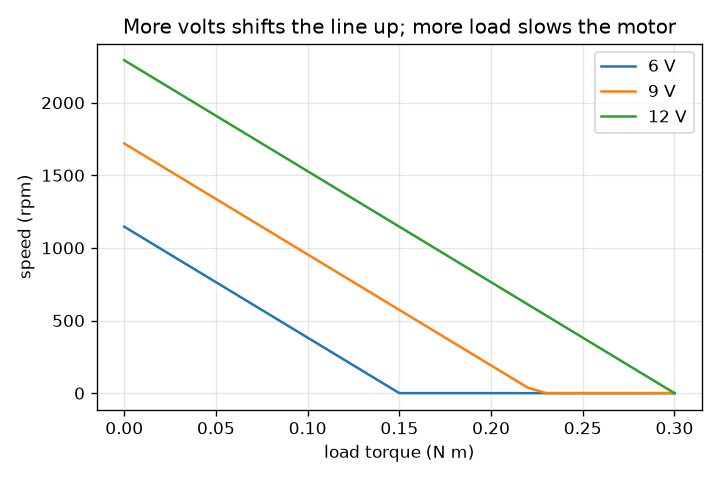
\includegraphics[width=0.85\linewidth]{figures/s01_speed_vs_load.png}\\\small Speed against load for 6, 9 and 12 V: heavier load, slower motor; more volts, faster motor.\end{center}

\subsection*{E. Worked example}
The 12 V motor (stall torque 0.30 N m, no-load speed 240 rad/s) drives a load of 0.12 N m. Find its speed in rad/s and rpm, and the mechanical power.
\begin{enumerate}[nosep]
\item Load as a fraction of stall: 0.12 / 0.30 = 0.4.
\item Speed = 240 x (1 - 0.4) = 144 rad/s.
\item rpm = 144 x 60 / (2 pi) = 1375 rpm (to 4 digits, 1375.1).
\item Power = torque x speed = 0.12 x 144 = 17.28 W.
\item Sanity check: the speed is between 0 and 240 rad/s, and the load is below the stall torque, so the motor turns.
\end{enumerate}
\textbf{Answer.} 144 rad/s, about 1375 rpm, delivering 17.28 W.

\subsection*{F. Questions}
\begin{enumerate}[nosep]
\item \textbf{Conceptual.} Why does a motor slow down when the load grows? Why does it never turn faster than the no-load speed?
\item \textbf{Numerical.} The 12 V motor drives a load of 0.21 N m. Find the speed in rad/s and rpm. Then find the load torque that gives exactly half the no-load speed.
\item \textbf{Graph and simulation interpretation.} In the speed-versus-load graph, what does the 6 V line do compared with the 12 V line? At what load does each reach zero speed?
\item \textbf{Design and optimisation challenge.} A load needs 0.15 N m at no less than 1000 rpm (104.7 rad/s). Can the 12 V motor do it? What is the lowest voltage in 0.5 V steps that does it?
\end{enumerate}

\section{Session 2: The DC motor model, power, and choosing a gearbox}

\subsection*{A. Real-world problem}
You must lift a 5 kg load at a steady pace with a small 12 V motor and a winch drum of radius 2 cm. The bare motor spins fast but is weak; a gearbox trades speed for torque. What gear ratio lifts the load at the speed you want without drawing too much current? (A simplified, low-voltage educational model, not a design tool.)

\subsection*{B. Concept and theory}
Two equations describe the motor. Electrical: the supply voltage V pushes a current I through the winding resistance R, and the spinning rotor makes a back voltage k\_e w that opposes it, so V = I R + k\_e w. Mechanical: torque is proportional to current, T = k\_t I. In SI units k\_t and k\_e are the same number k (N m/A is the same as V s/rad), because the electrical power that goes into the back voltage, k\_e w I, must come out as mechanical power T w = k\_t I w. Eliminating I gives the straight line T = k (V - k w) / R. At w = 0 this is the stall torque T\_stall = k V / R, with stall current V / R; at T = 0 it is the no-load speed w\_noload = V / k. Efficiency is mechanical output over electrical input, T w / (V I) = w / w\_noload for the ideal motor, and the output power T w is a parabola peaking at half the no-load speed, where the efficiency is exactly 50 percent. Real motors lose some torque to friction; with viscous friction b the line becomes T = T0 - a w with a = k\textasciicircum{}2/R + b, the peak moves slightly down and the efficiency at the peak falls below 50 percent. A gearbox of ratio N and efficiency eta turns motor torque T\_m and speed w\_m into output torque N eta T\_m and speed w\_m / N.

\begin{itemize}[nosep]
\item V: supply voltage (V)
\item I: winding current (A)
\item R: winding resistance (ohm)
\item k: motor constant, k\_t = k\_e (N m/A = V s/rad)
\item w: shaft speed (rad/s)
\item T: shaft torque (N m)
\item b: viscous friction coefficient (N m s/rad)
\item N, eta: gear ratio and gearbox efficiency (no unit)
\end{itemize}

\begin{equation*}
V=IR+k_e\omega,\qquad T=k_tI,\qquad k_t=k_e=k
\end{equation*}

\begin{equation*}
T=\frac{k\,(V-k\omega)}{R}=T_{\mathrm{stall}}\left(1-\frac{\omega}{\omega_{\mathrm{noload}}}\right),\quad T_{\mathrm{stall}}=\frac{kV}{R},\ \ \omega_{\mathrm{noload}}=\frac{V}{k}
\end{equation*}

\begin{equation*}
P_{\mathrm{in}}=VI,\qquad P_{\mathrm{out}}=T\omega,\qquad \eta_{\mathrm{motor}}=\frac{T\omega}{VI}=\frac{\omega}{\omega_{\mathrm{noload}}}\ \ (b=0)
\end{equation*}

\begin{equation*}
P_{\mathrm{out}}(\omega)=T_{\mathrm{stall}}\,\omega\left(1-\frac{\omega}{\omega_{\mathrm{noload}}}\right),\quad \omega^{*}=\frac{\omega_{\mathrm{noload}}}{2},\ \ P_{\max}=\frac{T_{\mathrm{stall}}\,\omega_{\mathrm{noload}}}{4}
\end{equation*}

\begin{equation*}
T_{\mathrm{out}}=N\eta_g T_m,\qquad \omega_{\mathrm{out}}=\frac{\omega_m}{N}
\end{equation*}

\begin{center}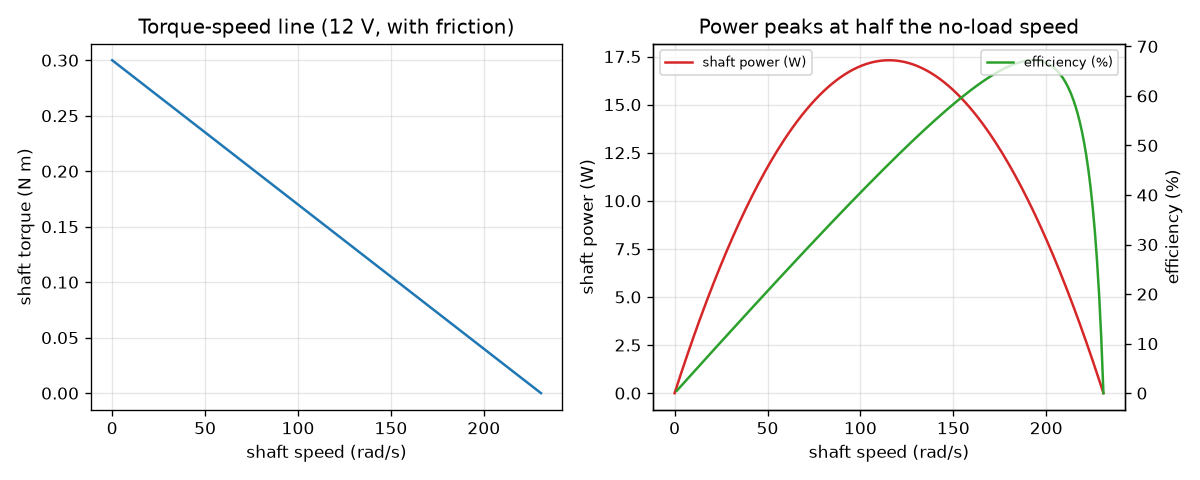
\includegraphics[width=0.85\linewidth]{figures/s02_curve_and_power.png}\\\small Torque-speed line (left), shaft power and efficiency against speed (right), with friction.\end{center}

\subsection*{E. Worked example}
For the motor V = 12 V, R = 2.0 ohm, k = 0.05 N m/A: find the stall torque, stall current, no-load speed, peak power and efficiency there. Then choose the best gear ratio for the winch (load torque 0.981 N m, drum speed at least 5 rad/s, current at most 1.5 A, gearbox efficiency 0.9, friction b = 5e-5).
\begin{enumerate}[nosep]
\item Stall torque = k V / R = 0.05 x 12 / 2 = 0.300 N m; stall current = V / R = 6 A.
\item No-load speed = V / k = 12 / 0.05 = 240 rad/s = 2292 rpm.
\item Ideal peak power = T\_stall x w\_noload / 4 = 0.3 x 240 / 4 = 18.00 W at 120 rad/s, where the efficiency is w / w\_noload = 50 percent.
\item With friction: a = k\textasciicircum{}2/R + b = 0.00125 + 0.00005 = 0.0013; the shaft line is T = 0.300 - 0.0013 w, which reaches zero at 230.8 rad/s. Peak power = 0.3 x 230.8 / 4 = 17.31 W at 115.4 rad/s; there I = (12 - 0.05 x 115.4) / 2 = 3.12 A, input power 37.4 W, so efficiency = 17.31 / 37.4 = 46.3 percent (below 50).
\item Load: the drum torque is 5 x 9.81 x 0.02 = 0.981 N m. For ratio N the motor must give T\_m = 0.981 / (0.9 N) and runs where 0.300 - 0.0013 w = T\_m.
\item Scanning ratios 5 to 60: N = 17 to 42 meet drum speed \textgreater{}= 5 rad/s and current \textless{}= 1.5 A. N = 16 draws 1.54 A (too much); N = 43 gives 4.91 rad/s (too slow).
\item Best efficiency in the window: N = 22. Motor torque 0.0496 N m, motor speed 192.7 rad/s (1840 rpm), drum speed 8.76 rad/s = 0.175 m/s, current 1.18 A, overall efficiency 60.5 percent.
\end{enumerate}
\textbf{Answer.} T\_stall = 0.300 N m, I\_stall = 6 A, w\_noload = 240 rad/s (2292 rpm); ideal peak 18.00 W at 120 rad/s and 50 percent efficiency, 17.31 W at 115.4 rad/s and 46.3 percent with friction. For the winch use N = 22 (allowed window 17 to 42): 8.76 rad/s, 1.18 A, 60.5 percent.

\subsection*{F. Questions}
\begin{enumerate}[nosep]
\item \textbf{Conceptual.} Why is the efficiency at maximum power below 50 percent in a real motor, and why is the best-efficiency speed higher than the best-power speed?
\item \textbf{Numerical.} A motor has V = 6 V, R = 1.5 ohm, k = 0.03 N m/A (no friction). Find the stall torque, stall current, no-load speed (rad/s and rpm) and peak mechanical power.
\item \textbf{Graph and simulation interpretation.} In the gear-ratio window graph, what happens to the output speed and to the current as the ratio grows from 17 to 42? Which limit decides the lower end of the window and which the upper end?
\item \textbf{Design and optimisation challenge.} Design: lift a 3 kg load on the same 2 cm drum at a drum speed of at least 8 rad/s with at most 1.5 A. Which ratios work and which would you choose? State the trade-off.
\end{enumerate}

\section{Session 3: A motor in time: simulation, PWM and sizing a robot drive}

\subsection*{A. Real-world problem}
A real motor does not jump to its steady speed. Switch it on and the current spikes first, because the rotor is still and there is no back voltage; then the speed climbs and the current falls. A robot also controls speed by switching the supply on and off very fast (PWM). And a robot that climbs a ramp must have the right motor and gearbox. Can we simulate all of this, trust the simulation, and use it to decide? (Low-voltage simplified lumped model, for education only: never wire a real motor or battery from this lesson alone.)

\subsection*{B. Concept and theory}
Add the two things Session 2 left out: the winding inductance L, which makes the current take time to change, and the inertia J of the rotor and load, which makes the speed take time to change. Electrical: L di/dt = V - R i - k w. Mechanical: J dw/dt = k i - b w - T\_load. These two coupled first-order equations have no neat formula in general, so we step through time with RK4 (Runge-Kutta 4): four slope samples per step, error shrinking with the fourth power of the step. Two time constants appear: tau\_e = L / R (2.5 ms here, fast) and tau\_m = J R / (k\textasciicircum{}2 + b R) (153.8 ms here, slow). Because tau\_e is much shorter than tau\_m, the speed follows a simple rise 1 - exp(-t / tau\_m) towards the steady speed from the Session 2 line. PWM switches the supply V fully on for a fraction D (the duty cycle) of each period and off for the rest; the motor sees the average voltage D V, and since the rotor is slow its speed ripple is tiny, but the current ripple is about D (1 - D) V / (L f) for PWM frequency f. Energy must balance: the electrical energy in equals heat in the winding (R i\textasciicircum{}2) plus friction heat (b w\textasciicircum{}2) plus the work done on the load (T\_load w) plus the stored energy 1/2 J w\textasciicircum{}2 (rotor) and 1/2 L i\textasciicircum{}2 (inductor). The starting margin of a geared drive is the torque it gives at stall, N eta k V / R, divided by the torque the task needs. A locked rotor (stall) has w = 0, so the current tends to V / R and the winding heat is R i\textasciicircum{}2 = V\textasciicircum{}2 / R.

\begin{itemize}[nosep]
\item L: winding inductance (H)
\item J: rotor plus load inertia (kg m\textasciicircum{}2)
\item i, w: current and speed (the state) (A, rad/s)
\item tau\_e, tau\_m: electrical and mechanical time constants (s)
\item D: PWM duty cycle, 0 to 1 (no unit)
\item f: PWM frequency (Hz)
\item m, r, theta, c: robot mass, wheel radius, slope angle, rolling-resistance coefficient (kg, m, degrees, no unit)
\item dt: RK4 time step (s)
\end{itemize}

\begin{equation*}
L\frac{di}{dt}=V-Ri-k\omega,\qquad J\frac{d\omega}{dt}=ki-b\omega-T_{\mathrm{load}}
\end{equation*}

\begin{equation*}
\tau_e=\frac{L}{R},\qquad \tau_m\approx\frac{JR}{k^2+bR},\qquad \omega(t)\approx\omega_{ss}\left(1-e^{-t/\tau_m}\right)
\end{equation*}

\begin{equation*}
\omega_{ss}=\frac{kV/R-T_{\mathrm{load}}}{k^2/R+b},\qquad V_{\mathrm{avg}}=DV,\qquad \Delta i\approx\frac{D(1-D)V}{Lf}
\end{equation*}

\begin{equation*}
\int Vi\,dt=\int Ri^2\,dt+\int b\omega^2\,dt+\int T_{\mathrm{load}}\omega\,dt+\tfrac12J\omega^2+\tfrac12Li^2
\end{equation*}

\begin{equation*}
F=mg\,(\sin\theta+c\cos\theta),\qquad T_{\mathrm{wheel}}=\frac{Fr}{n},\qquad T_m=\frac{T_{\mathrm{wheel}}}{N\eta}
\end{equation*}

\begin{center}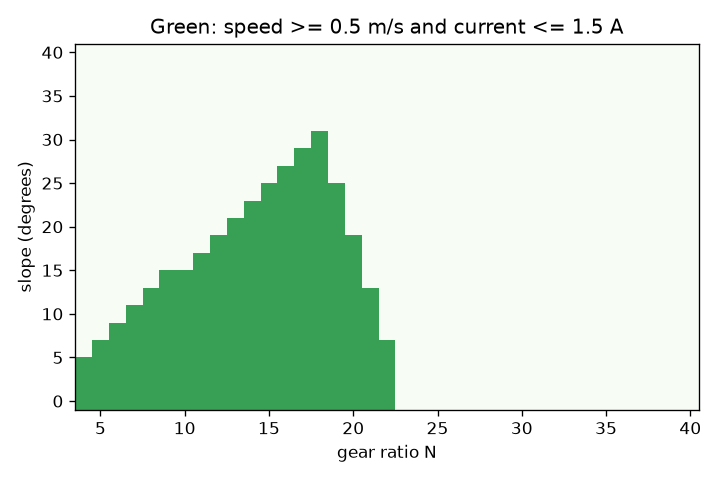
\includegraphics[width=0.85\linewidth]{figures/s03_sizing_sweep.png}\\\small Sizing sweep for the 8 kg robot: green marks gear ratio and slope combinations that meet speed and current limits.\end{center}

\subsection*{E. Worked example}
A 12 V motor (R = 2.0 ohm, L = 5 mH, k = 0.05, b = 5e-5, J = 2e-4 kg m\textasciicircum{}2) starts from rest with no load. Find tau\_e, tau\_m, the steady speed and current, then check them against the RK4 simulation and the energy balance.
\begin{enumerate}[nosep]
\item tau\_e = L / R = 0.005 / 2 = 2.5 ms.
\item tau\_m = J R / (k\textasciicircum{}2 + b R) = 2e-4 x 2 / (0.0025 + 0.0001) = 4e-4 / 0.0026 = 0.1538 s.
\item Steady speed = (k V / R) / (k\textasciicircum{}2/R + b) = 0.3 / 0.0013 = 230.77 rad/s; steady current = b w / k = 5e-5 x 230.77 / 0.05 = 0.231 A.
\item The first-order approximation says 63.2 percent of the final speed (145.8 rad/s) is reached at t = tau\_m = 153.8 ms.
\item Simulation (RK4, dt = 0.1 ms): the speed reaches 63.2 percent at 154.0 ms, within 0.2 percent of the formula; the current peaks at 5.70 A (below the stall limit V / R = 6 A) at 10.7 ms.
\item Energy: in one second the supply delivers 13.41 J; the sum of winding heat, friction heat, stored kinetic and magnetic energy matches it with a residual of about 5e-9 J.
\end{enumerate}
\textbf{Answer.} tau\_e = 2.5 ms, tau\_m = 153.8 ms, steady 230.77 rad/s and 0.231 A; the simulation gives 154.0 ms for 63.2 percent speed, a start-up current peak of 5.70 A, and conserves energy to 5e-9 J.

\subsection*{F. Questions}
\begin{enumerate}[nosep]
\item \textbf{Conceptual.} Why is the speed ripple in PWM almost zero while the current ripple is clearly visible?
\item \textbf{Numerical.} The load inertia is doubled to J = 4e-4 kg m\textasciicircum{}2. Find the new mechanical time constant, and the time for the speed to reach 63.2 percent. How does the steady speed change?
\item \textbf{Graph and simulation interpretation.} In the PWM current graph, what happens to the ripple when you double the frequency from 1000 to 2000 Hz at D = 0.5? What does the hand estimate predict and why does it fall?
\item \textbf{Design and optimisation challenge.} Design: a 5 kg robot with the same wheels (radius 0.05 m, two driven wheels, c = 0.03) must climb 25 degrees at 0.5 m/s or more with at most 1.5 A per motor and a starting margin of at least 1.5. Which gear ratios work? Which would you choose?
\end{enumerate}

\section{Real-world mini-project}
\textbf{Size a motor and gearbox for a robot wheel climbing a slope.} A robot of 8 kg runs on two driven wheels of radius 0.05 m (rolling resistance coefficient 0.03). Each wheel has one of the 12 V motors from the lessons and a gearbox of efficiency 0.9. The robot must climb a 25 degree ramp at 0.5 m/s or more, each motor may draw at most 1.5 A continuously, and the gearbox must give a starting-torque margin of at least 1.5. Use \texttt{window} and \texttt{wheel\_drive} from Session 3 to list the allowed gear ratios, pick one with an engineering argument, and confirm your pick with \texttt{climb\_sim}.

\section{The path ahead}
\begin{enumerate}[nosep]
\item \textbf{Session 4: Climb steeper: the 35 degree drive.} A drive study that extends \texttt{window} to compare motors, supply voltages and gear stages.
\item \textbf{Session 5: Hold the speed: closed-loop control.} A PI speed controller that sets the duty cycle from the speed error, added to the time-domain simulation.
\item \textbf{Session 6: Measure your own motor.} A parameter-fitting script and a bench procedure for a real hobby motor.
\item \textbf{Session 7: Battery sag and a thermal limit.} A battery model and a one-state thermal model for the winding, wired into the simulation.
\item \textbf{Session 8: Downhill and regenerative braking.} A descent simulation of the robot with the motor acting as a generator.
\end{enumerate}

\section{Answers and hints}

\subsection*{Session 1}
\begin{enumerate}[nosep]
\item \textbf{Conceptual.} Hint: Where does the straight line cross the speed axis, and what torque is left there? Solution: The motor can only give the torque the line allows at its present speed. A heavier load asks for more torque, which the line only offers at a lower speed, so the motor settles slower. At the no-load speed the line says the motor gives zero torque, so there is nothing left to push it faster. A load of zero therefore gives the highest speed, the no-load speed.
\item \textbf{Numerical.} Hint: Use speed = 240 x (1 - load / 0.30). Half speed means (1 - load / 0.30) = 0.5. Solution: Fraction of stall: 0.21 / 0.30 = 0.7, so speed = 240 x 0.3 = 72 rad/s, which is 72 x 60 / (2 pi) = 687.5 rpm. Half the no-load speed (120 rad/s) needs 1 - load / 0.30 = 0.5, so load = 0.15 N m. Sanity check: 0.15 is half of the stall torque, as the straight line demands.
\item \textbf{Graph and simulation interpretation.} Hint: Remember that both the stall torque and the no-load speed scale with voltage. Solution: The 6 V line starts at half the speed (1146 rpm against 2292 rpm at no load) and reaches zero speed at half the load, 0.15 N m instead of 0.30 N m. The 9 V line lies in between, stalling at 0.225 N m. So a lower voltage shrinks both the top speed and the load the motor can carry.
\item \textbf{Design and optimisation challenge.} Hint: At voltage V the line has stall torque 0.025 V and no-load speed 20 V. Solve speed = 20 V (1 - 0.15 / (0.025 V)) \textgreater{}= 104.7. Solution: At 12 V the speed is 240 x (1 - 0.15 / 0.30) = 120 rad/s = 1146 rpm, which is above 1000 rpm, so yes. The speed at voltage V is 20 V - 120, so 20 V - 120 \textgreater{}= 104.7 gives V \textgreater{}= 11.24; in 0.5 V steps the lowest voltage is 11.5 V. Trade-off: the motor then runs close to its limits; a motor with a bigger stall torque would run cooler.
\end{enumerate}

\subsection*{Session 2}
\begin{enumerate}[nosep]
\item \textbf{Conceptual.} Hint: Efficiency of the ideal motor is w / w\_noload. What does friction subtract from the shaft power but not from the electrical input? Solution: For the ideal motor, efficiency is the speed fraction w / w\_noload, exactly 0.5 at the speed of peak power. Friction takes a share of the torque, so the shaft power is less than k I w, while the electrical input V I is unchanged, so the efficiency at that speed drops below 50 percent (46.3 percent here). Efficiency keeps rising with speed because the current (and so the resistive loss) falls as the back voltage grows, while power falls to zero at no load. Best efficiency (67 percent here) is therefore near 193 rad/s, well above the 115 rad/s of peak power.
\item \textbf{Numerical.} Hint: T\_stall = k V / R, w\_noload = V / k, P\_max = T\_stall w\_noload / 4. Solution: T\_stall = 0.03 x 6 / 1.5 = 0.12 N m. I\_stall = 6 / 1.5 = 4 A. w\_noload = 6 / 0.03 = 200 rad/s = 200 x 60 / (2 pi) = 1910 rpm. P\_max = 0.12 x 200 / 4 = 6.0 W at 100 rad/s. Sanity check: P\_max is 6 W while the electrical power at stall would be 24 W, a quarter of it, as expected.
\item \textbf{Graph and simulation interpretation.} Hint: Look at which curve crosses its flat limit line at each end. Solution: As the ratio grows the output speed falls (10.7 to 5.0 rad/s) and the current falls too (1.46 to 0.73 A), because the motor torque needed falls as 1 / N. The lower end of the window, N = 17, is set by the current limit (N = 16 draws 1.54 A); the upper end, N = 42, is set by the speed requirement (N = 43 gives only 4.91 rad/s).
\item \textbf{Design and optimisation challenge.} Hint: Load torque = 3 x 9.81 x 0.02. Scan N with the Session 2 functions \texttt{operating\_point} and \texttt{choose\_ratio}. Solution: Load torque = 0.5886 N m. The window is N = 10 to 26. The most efficient is N = 13 (14.77 rad/s, 1.20 A, 60.5 percent efficiency). Trade-off: a low ratio (near 10) lifts faster but draws more current and heats the motor; a high ratio (near 26) is gentle on the motor but barely meets the speed requirement and wastes speed capability. Choosing about 13 to 15 keeps margin on both limits.
\end{enumerate}

\subsection*{Session 3}
\begin{enumerate}[nosep]
\item \textbf{Conceptual.} Hint: Compare the PWM period (1 ms) with tau\_e (2.5 ms) and tau\_m (153.8 ms). Solution: The inductance makes the current respond over a time tau\_e = 2.5 ms, comparable with the 1 ms PWM period, so the current visibly rises during the on-time and falls during the off-time. The rotor's inertia makes the speed respond over tau\_m = 153.8 ms, 150 times longer than the period, so it averages the torque pulses and barely moves (0.02 rad/s peak to peak). The mean speed is therefore the speed at the average voltage D V.
\item \textbf{Numerical.} Hint: tau\_m = J R / (k\textasciicircum{}2 + b R). Steady speed does not contain J. Solution: tau\_m = 4e-4 x 2 / 0.0026 = 0.3077 s (twice as long). The simulation gives 0.3078 s for 63.2 percent of the final speed. The steady speed 230.77 rad/s is unchanged, since J appears only in the equation for how fast the speed changes, not in the balance where the derivatives are zero.
\item \textbf{Graph and simulation interpretation.} Hint: Use the estimate D (1 - D) V / (L f). Solution: The estimate gives 0.25 x 12 / (0.005 x 1000) = 0.60 A at 1 kHz and 0.30 A at 2 kHz: the ripple halves, because each on or off interval is half as long so the current has half as much time to change. The simulation gives 0.598 A and 0.300 A. Higher frequency means smoother current but more switching loss in a real driver, which the model does not include.
\item \textbf{Design and optimisation challenge.} Hint: Call \texttt{window(25, robot=\{'m': 5.0\})} and \texttt{wheel\_drive} for the ratios at the edges. Solution: The window is N = 10 to 20 (N = 9 draws 1.54 A, N = 21 gives only 0.496 m/s). The most efficient is N = 12: 0.798 m/s, 1.21 A, starting margin 5.9, efficiency 60.5 percent. I would choose about 12 to 14: well inside both limits, faster than needed. Trade-off: a higher ratio runs cooler and has more torque margin but is slower and wastes efficiency; a lower ratio is faster but near the current limit.
\end{enumerate}

\section{How to join}
Read \texttt{CONTRIBUTING.md} in the repository, then pick an issue labelled \texttt{good first issue}. Repository: \url{https://github.com/KrunalPanchal1995/opendcmotor}

\end{document}
